\documentclass[conference]{IEEEtran}

\usepackage{cite}
\usepackage{amsfonts,amsmath,amssymb,amsthm,booktabs,color,enumitem,graphicx}


% correct bad hyphenation here
\hyphenation{op-tical net-works semi-conduc-tor}


\begin{document}

\title{Pipeline for continuous deployment and continuous experimentation}

\author{\IEEEauthorblockN{Olli Rissanen}
\IEEEauthorblockA{Department of Computer Science\\
University of Helsinki\\
Helsinki, Finland\\
Email: olli.rissanen@helsinki.fi}}

% make the title area
\maketitle


\begin{abstract}
Currently more and more software companies are moving to lean practices, which often include shorter delivery cycles and thus shorter feedback loops. However, to achieve continuous customer feedback and to eliminate work that doesn't generate value, even shorter cycles are required. In continuous deployment the software functionality is deployed continuously at customer environment. This process includes both automated builds and automated testing, but also automated deployment. This adds more elements to the development pipeline, which often in a lean team consists of a version control system and a continuous integration server. Automating the whole process minimizes the time required for implementing new features in software, and allows for faster customer feedback. However, adopting continuous deployment doesn't necessarily mean that more value is created for the customer. 

Continuous deployment attempts to deliver an idea to users as fast as possible. Continuous experimentation instead attempts to validate that it is, in fact, a good idea.

\end{abstract}
% IEEEtran.cls defaults to using nonbold math in the Abstract.
% This preserves the distinction between vectors and scalars. However,
% if the conference you are submitting to favors bold math in the abstract,
% then you can use LaTeX's standard command \boldmath at the very start
% of the abstract to achieve this. Many IEEE journals/conferences frown on
% math in the abstract anyway.

% no keywords




% For peer review papers, you can put extra information on the cover
% page as needed:
% \ifCLASSOPTIONpeerreview
% \begin{center} \bfseries EDICS Category: 3-BBND \end{center}
% \fi
%
% For peerreview papers, this IEEEtran command inserts a page break and


% creates the second title. It will be ignored for other modes.
\IEEEpeerreviewmaketitle

%Perusteet

%Kiinnostava
%Innostava
%Tehtävissä

%Määrittele
% Tutkimusongelma, siis mitä haluat ymmärtää tai selvittää
% Tavoitteet
% Menetelmät
% Rajaus

%Mahdollisia toteutustapoja
% Vertaile kahta tai useampaa lähestymistapaa
% Etsi empiiristä todistusaineistoa jonkin väitteen puolesta tai sitä vastaan
% Kuvaa tapausyrityksen tilanne ja vertaile kirjallisuuteen
%

%Haasteet

%In fact, one sign of a good application architecture is that it allows the application
%to be run without much trouble on a development machine.

\section{Introduction} %why is this problem interesting?
Continuous deployment is an extension to continuous integration, where the software functionality is deployed frequently at customer environment. While continuous integration defines a process where the work is automatically built, tested and frequently integrated to mainline \cite{fowler2006continuous}, often multiple times a day, continuous deployment adds automated acceptance testing and deployment. The purpose of continuous deployment is that as the deployment process is completely automated, it reduces human error, documents required for the build and increases confidence that the build works \cite{cdbook}. %Explain pipeline here

An important part of continuous deployment is the deployment pipeline. A deployment pipeline can be loosely defined as a consecutively executed set of validations that a software has to pass such before it can be released. The deployment pipeline is therefore an automated implementation of the application's build, deploy, test and release process \cite{cdbook}. Common components of the deployment pipeline are a version control system and an automated test suite.

In an agile process software release is done in periodic intervals \cite{cockburn2002agile}. Compared to waterfall model it introduces multiple releases throughout the development. Continuous deployment, on the other hand, attemps to keep the software ready for release at all times during development process \cite{cdbook}. Instead of stopping the development process and creating a build as in an agile process, the software is continuously deployed to customer environment. This doesn't mean that the development cycles in continuous deployment are shorter, but that the development is done in a way that makes the software always ready for release.

It should also be made clear that continuous delivery differs from continous deployment. Refer to Fig. \ref{fig1} for a visual representation of differences in continuous integration, delivery and deployment. Both include automated deployment to a staging environment. Continuous deployment includes deployment to a production environment, while in continuous delivery the deployment to a production environment is done manually. The purpose of continuous delivery is to prove that every build is proven deployable \cite{cdbook}. While it necessarily doesn't mean that teams release often, keeping the software in a state where a release can be made instantly is often seen beneficial.

Adopting a continuous deployment process doesn't necessarily mean that more value is delivered to a customer. Avinash Kaushik states in his Experimentation and Testing primer \cite{kaushik} that "80\% of the time you/we are wrong about what a customer wants". Mike Moran also found similar results in his book Do It Wrong Quickly, stating that Netflix considers 90\% of what they try to be wrong. A way to tackle this issue is to adopt a process of continuous experimentation, where the entire R\&D system responds and acts based on instant customer feedback, and where actual deployment of software functionality is seen as a way of experimenting and testing what the customer needs \cite{olsson2012climbing}.
 
Continuous deployment attempts to deliver an idea to users as fast as possible. Continuous experimentation instead attempts to validate that it is, in fact, a good idea. In continuous experimentation the organisation runs controlled experiments to guide the R\&D process. %Mitä continous experimentation tekee?
As the experiments are run in a regular fashion, it is only natural to attempt to integrate experiments to the deployment pipeline, and to change the development process in such fashion that functionality is developed based on some actual data. The operational changes required for a deployment pipeline to support continuous experimentation include %what?

%Continuous experimentation requires operational changes to the deployment pipeline. 

In this paper we're investigating %Main research question: How to integrate conducting experiments to the development process?

This paper is organized as follows.
\begin{figure}[!t]
	\centering
	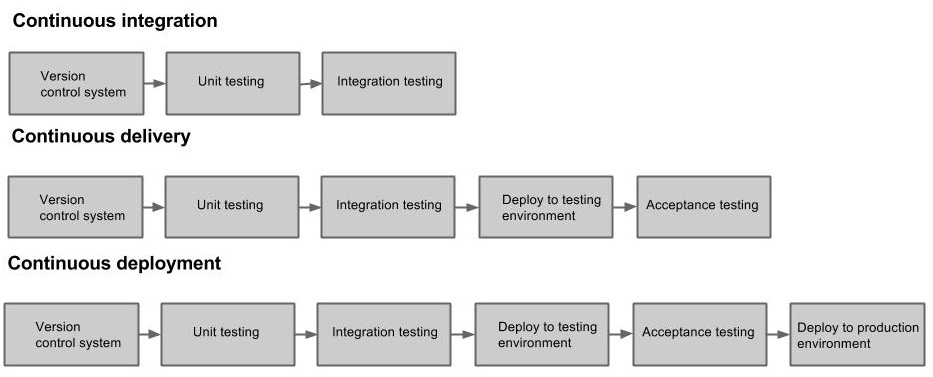
\includegraphics[width=3.5in]{rtvd.jpg}
	\caption{Continuous integration, delivery and deployment}
	\label{fig1}
\end{figure}

\section{Methods} %how did I find the papers? %TODO: UPDATE THIS


%Kerro tarkemmin kuin vaan mitä hakuja tehtiin
Searches were performed using the keywords shown in Table I. The searches were performed during February and March 2014 using IEEE Xplore (http://ieeexplore.ieee.org/‎) and Google Scholar (http://scholar.google.com/) search engines. Final papers were downloaded from the publishers web sites, if available. Plenty of research concerning software release management, release planning and iterative release planning were found, but the focus on architectural qualities appeared sparsely.  
\begin{center}
\begin{table}
    \caption{Keywords used for searching research materials.}
    \begin{tabular}{ | p{2cm} | p{2cm} | p{3.5cm} |}
    \hline
    Search string & Search engine & Article \\ \hline
    software release management & Google Scholar & Software Release Management \\ \hline
	release planning architecture & IEEE Xplore & Importance of Software Architecture during Release Planning \\ \hline
	deployment production line & IEEE Xplore & The deployment production line \\ \hline
	iterative release planning architecture & IEEE Xplore & Analysis and Management of Architectural Dependencies in Iterative Release Planning \\ \hline
    \end{tabular}
    \end{table}
\end{center}
As searches regarding architecture in continuous delivery and deployment returned no results, a decision was made to instead focus on research related to architectural features and issues in releases, and then attempting to apply those findings to continuous deployment. Articles regarding release management, release planning, iterative release planning and deployment pipeline were chosen for this purpose.

\section{Results} %Pure analysis on the papers

A deployment pipeline for continuous deployment consists of the phases a build has to pass in order for it to be deployed. A pipeline for continuous experimentation, on the other hand, consists of the steps required to design, execute and analyse an experiment. The cycle of continuous experimentation resembles the build-measure-learn cycle of lean startup \cite{ries2011lean}. In continuous experimentation, the main process is to deploy new functionality, measure usage and other performance metrics and subsequently to use the collected data to drive development \cite{bosch2012building}.

Lean startup \cite{ries2011lean} %MVP

Stairway to heaven Olsson \cite{olsson2012climbing}

Building products as innovative \cite{bosch2012building}

Practical guide \cite{kohavi2007practical}

Deployment production line \cite{humble2006deployment}

\subsection{Pipeline for continuous deployment}	

The primary purpose of continuous deployment is to improve the process of software delivary. This is done by automating the whole deployment process, since unless deployments are automated, errors will occur every time they're performed \cite{cdbook}. The components of a deployment pipeline typically are a version control system and an automated test suite consisting of unit tests, integration tests and acceptance tests. 

Humble and Farley define the deployment pipeline as a set of stages, which cover the path from a committed change to a build \cite{cdbook}. Refer to Fig. \ref{fig2} for a graphical representation of a basic deployment pipeline. The commit stage compiles the build and runs code analysis, while acceptance stage runs an automated test suite that asserts the build works at both functional and nonfunctional level. From there on, builds to different environments can be deployed either automatically or by a push of a button.
\begin{figure}[!t]
	\centering
	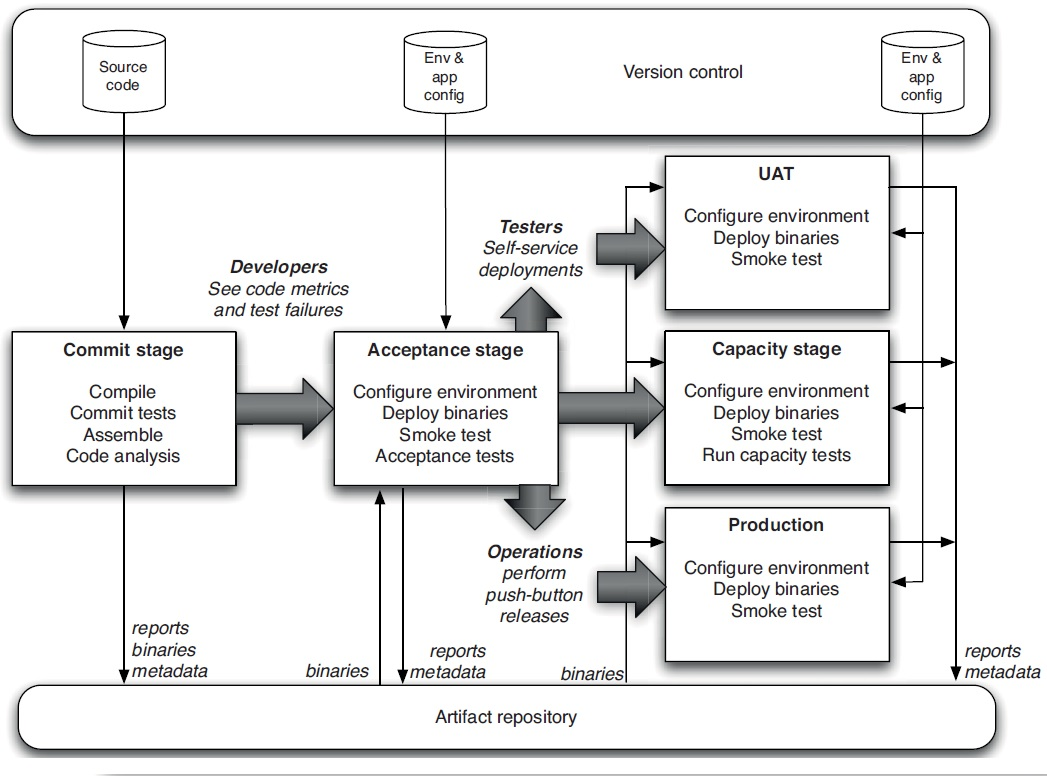
\includegraphics[width=3.5in]{pipeline.jpg}
	\caption{A basic deployment pipeline \cite{cdbook}.}
	\label{fig2}
\end{figure}

Humble et al. define four principles that should be followed when attempting to automate the deployment process \cite{humble2006deployment}. The first principle states that "Each build stage should deliver working software". As software often consists of different modules with dependencies to other modules, a change to a module could trigger builds of the related modules as well. Humble et al. argue that it is better to keep builds separate so that each discrete module could be built individually. The reason is that triggering other builds can be inefficient, and information can be lost in the process. The information loss is due to the fact that connection between the initial build and later builds is lost, or at least causes a lot of unnecessary work spent in tracing the triggering build. 

The second principle states that "Deploy the same artifacts in every environment". This creates a constraint that the configuration files must be kept separate, as different environments often have different configurations. Humble et al. state that a common anti-pattern is to aim for 'ultimate configurability', and instead the simplest configuration system that handles the cases should be implemented.

Another principle, which is the main element of continuous deployment, is to "Automate testing and deployment". Humble et al. argue that the application testing should be separated out, such that stages are formed out of different types of tests. This means that the process can be aborted if a single stage fails. They also state that all states of deployment should be automated, including deploying binaries, configuring message queues, loading databases and related deployment tasks. Humble et al. mention that it might be necessary to split the application environment into $slices$, where each slice contains a single instance of the application with predetermined set of resources, such as ports and directories. $Slices$ make it possible to replicate an application multiple times in an environment, to keep distinct version running simultaniously. Finally, the environment can be smoke tested to test the environments capabilities and status.

The last principle states "Evolve your production line along with the application it assembles". Humble et al. state that attempting to build a full production line before writing any code doesn't deliver any value, so the production line should be built and modified as the application evolves. 

%Humble et al. define four principles that guide in implementing the deployment pipeline \cite{humble2006deployment}. The first principle states that "Each build stage should deliver working software". 

%The second principle states "Deploy the same artifacts in every environment - manage your runtime configuration separately".

%The third principle states "Automate testing and deployment - use several independent testing stages".

%The fourth principle states "Evolve your production line along with the application it assembles".

"A deployment pipeline is an automated implementation of your application's build, deploy, test and release process" \cite{cdbook}.

\begin{figure}[!t]
	\centering
	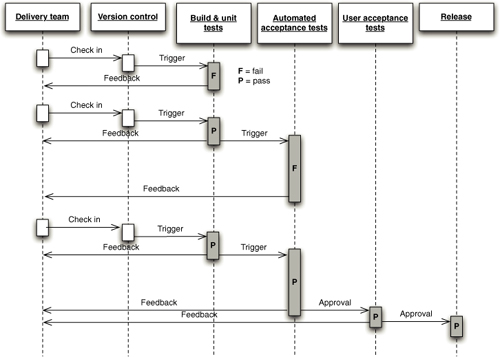
\includegraphics[width=3.5in]{developmentprocess.jpg}
	\caption{Components of the development process \cite{cdbook}.}
	\label{fig3}
\end{figure}

\subsection{Experimentation}

An experiment is essentially a procedure to confirm the validity of a hypothesis. In software engineering context, experiments attempt to answer questions such as which features are necessary for a product to succeed, what should be done next and which customer opinions should be listened to. According to Jan Bosch, "The faster the organization learns about the customer and the real world operation of the system, the more value it will provide" \cite{bosch2012building}. Most organizations have many ideas, but the return-on-investment for many may be unclear and the evaluation itself may be expensive \cite{kohavi2007practical}. I

In Lean startup methodology \cite{ries2011lean} experiments consist of Build-Measure-Learn cycles, and are tightly connected to visions and the business strategy. The purpose of a Build-Measure-Learn cycle is to turn ideas into products, measure how customers respond to the product and then to either pivot or persevere the chosen strategy. The cycle starts with forming a hypothesis and building a minimum viable product (MVP) with tools for data collection. Once the MVP has been created, the data is analyzed and measured in order to validate the hypothesis. To persevere with a chosen strategy means that the experiment proved the hypothesis correct, and the full product or feature can is implemented. However, if the experiment proved the hypothesis wrong, the strategy is changed based on the implications of a false hypothesis.

Jan Bosch has widely studied continuous experimentation, or innovation experiment systems, as a basis for development. The primary issue he found is that "experimentation in online software is often limited to optimizing narrow aspects of the front-end of the website through A/B testing and inconnected, software-intensive systems experimentation, if applied at all, is ad-hoc and not systematically applied" \cite{bosch2012building}.

Fig. \ref{fig4} introduces different stages and scopes for experimentation. For each stage and scope combination, an example technique to collect product performance data is shown. As startups often start new products and older companies instead develop new features, experiments must be applied in the correct context. Bosch states that for a new product deployment, putting a minimal viable product as rapidly as possible in the hands of customers is essential \cite{bosch2012building}. After the customers can use the product, it is often not yet monetizable but is still of value to the customer. %TODO: loppuun tää
\begin{figure}[!t]
	\centering
	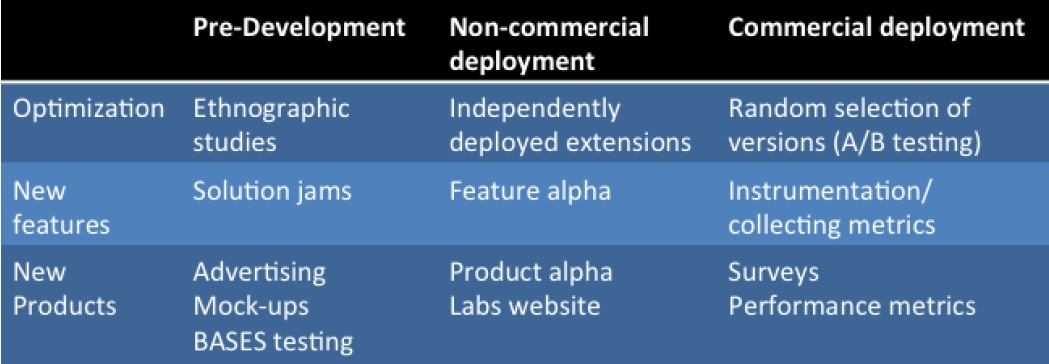
\includegraphics[width=3.5in]{bosch.jpg}
	\caption{Scopes for experimentation\cite{bosch2012building}.}
	\label{fig4}
\end{figure}
Crook et al. investigated the common pitfalls encountered when running controlled experiments on the web \cite{crook2009seven}, which are listed in Table II. The Overall Evaluation Criteria (OEC) used in the first pitfall is a quantitative measure of the experiment's objective. In experimental design, Control is a term used for the existing feature or a process, while a Treatment is used to describe a modified feature or a process. As a motivator for the first pitfall, Crook et al. introduce an experiment where the OEC was set to the time spent on a page which contains articles. The OEC increased in the experiment implementation, satisfying the objective. However, it was soon realized that the longer time spent on a page might have been caused by confusion of the users, as a newly introduced widget was used less often than a previous version of it. 

Aside from picking a correct OEC, common pitfalls deal with the correct use of statistical analysis, robot users such as search engine crawlers, and the importance of audits and control.
\begin{center}
\begin{table}
    \caption{Pitfall to avoid when running controlled experiments on the web \cite{crook2009seven}.}
    \begin{tabular}{ | p{1cm} | p{6cm} |}
    \hline
	Pitfall 1 & Picking an OEC for which it is easy to beat the control by doing something clearly “wrong” from a business perspective \\ \hline
	Pitfall 2 & Incorrectly computing confidence intervals for percent change and for OECs that involve a nonlinear combination of metrics \\ \hline
	Pitfall 3 & Using standard statistical formulas for computations of variance and power \\ \hline
	Pitfall 4 & Combining metrics over periods where the proportions assigned to Control and Treatment vary, or over subpopulations sampled at different rates \\ \hline
	Pitfall 5 & Neglecting to filter robots \\ \hline
	Pitfall 6 & Failing to validate each step of the analysis pipeline and the OEC components \\ \hline
	Pitfall 7 & Forgetting to control for all differences, and assuming that humans can keep the variants in sync \\ \hline
    \end{tabular}
    \end{table}
\end{center}

Experimentation doesn't necessarily require development of software.

%Implementing an experiment on a website involves two components. The first component is the randomization algorithm, which is a function that maps users to variants. The second
%component is the assignment method, which uses the output of the randomization algorithm to determine the experience that each user will see on the website. During the experiment, observations must be collected, and data needs to be aggregated and analyzed \cite{kohavi2007practical}

\subsection{Pipeline for continous experimentation}

A system with continuous experimentation must be able to release minimum viable products with integrated data collection instruments in a rapid manner. 

Kohavi et al. investigate the practical implementations of controlled experiments on the web \cite{kohavi2007practical}, and state that the implementation of an experiment involves two components. The first component is a randomization algorithm, which is used to map users to different variants of the product in question. The second component is an assignment method which, based on the output of the randomization algorithm, determines the contents that each user are shown. The observations then need to be collected, aggregated and analyzed to validate a hypothesis. Kohavi et al. also state that most existing data collection systems are not designed for the statistical analyses that are required to correctly analyze the results of a controlled experiment.

The components introduced by Kohavi et al. are aimed primarily for A/B testing on websites. 

%The components of a pipeline for continuous experimentation should include a 


%Split this to themes instead of papers

\section{Discussion} %Own speculation

The quantitative measure must be correct (pitfall)

What kind of elements need to be added to the deployment pipeline based on these papers?

The pipeline for continuous deployment

The pipeline for continuous experimentation

Based on the features required by .., a set of restrictions can be ..

Restrictions
#1 Running an experiment should be optional, and deploying without experimenting must be made possible

\section{Future research} %Self-explanatory
\section{Conclusion} %Short wrap-up. Contains the key points


\bibliography{IEEEabrv,references}{}
\bibliographystyle{IEEEtran}
% trigger a \newpage just before the given reference
% number - used to balance the columns on the last page
% adjust value as needed - may need to be readjusted if
% the document is modified later
%\IEEEtriggeratref{8}
% The "triggered" command can be changed if desired:
%\IEEEtriggercmd{\enlargethispage{-5in}}

% references section

% can use a bibliography generated by BibTeX as a .bbl file
% BibTeX documentation can be easily obtained at:
% http://www.ctan.org/tex-archive/biblio/bibtex/contrib/doc/
% The IEEEtran BibTeX style support page is at:
% http://www.michaelshell.org/tex/ieeetran/bibtex/

% argument is your BibTeX string definitions and bibliography database(s)
%\bibliography{IEEEabrv,../bib/paper}
%
% <OR> manually copy in the resultant .bbl file
% set second argument of \begin to the number of references
% (used to reserve space for the reference number labels box)
%\begin{thebibliography}{1}

%\bibitem{IEEEhowto:kopka}
%H.~Kopka and P.~W. Daly, \emph{A Guide to \LaTeX}, 3rd~ed.\hskip 1em plus
%  0.5em minus 0.4em\relax Harlow, England: Addison-Wesley, 1999.

%\end{thebibliography}




% that's all folks
\end{document}


